\chapter{Entwicklung des Prototpys für Visual Studio Code}
\label{cha:EntwicklungVsCode}

\section{Design}
\label{sec:EntwicklungVsCode_Design}

Um das in Kapitel \ref{cha:Prototyp} beschriebene Plugin in VS Code
zu entwickeln, werden die Komponenten verwendet, die auch in 
Abbildung \ref{fig:diagram_VSCodeDesign-Simplified} abgebildet sind.
\begin{figure}
    \centering
    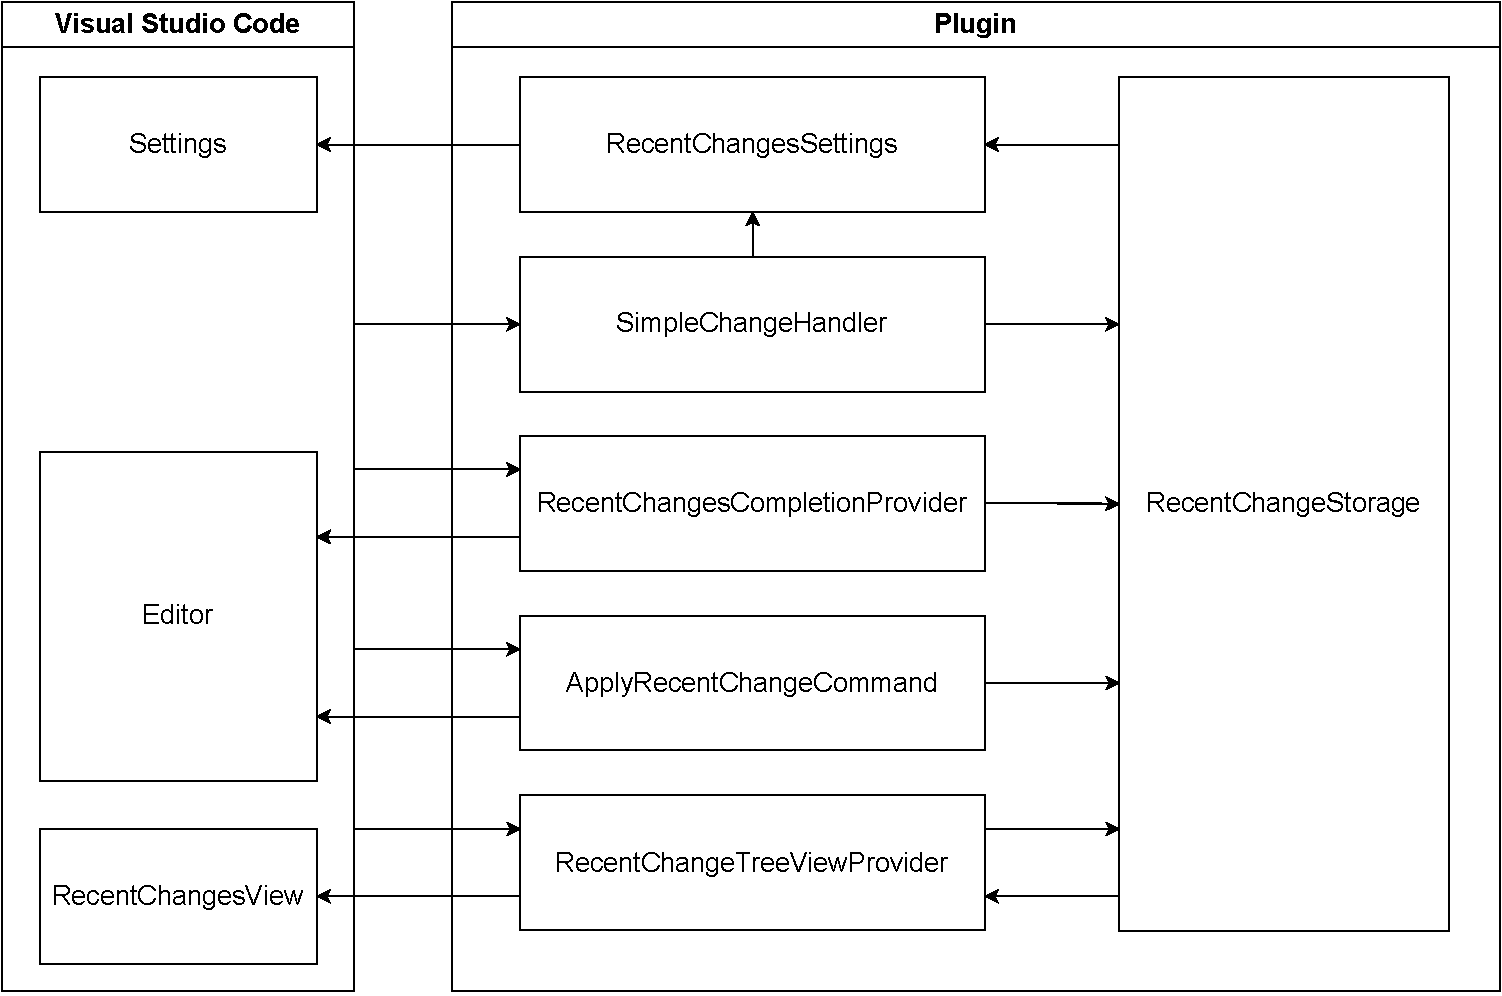
\includegraphics[width=.95\textwidth]{diagram_VSCodeDesign-Simplified}
    \caption{Stark vereinfachte Übersicht über das Design des Plugins in  VS Code.}
    \label{fig:diagram_VSCodeDesign-Simplified}
\end{figure}  

Das Herzstück des Plugins sind der \emph{SimpleChangeHandler} und
der \emph{RecentChangeStorage}. Der \emph{SimpleChangeHandler} hat die Aufgabe,
alle Veränderungen im geöffneten Dokument zu analysieren. Falls es sich um
eine verarbeitbare Veränderung handelt, wird diese im \emph{RecentChangeStorage}
gespeichert. Der \emph{RecentChangeStorage} bietet Methoden um die
gespeicherten Änderungen abzufragen und kümmert sich auch selber um das
Löschen von veralteten Änderungen.

Die Klasse \emph{RecentChangesSettings} bietet Zugriffsmethoden an,
um die von VS Code angebotenen Einstellungen abzufragen. Über sie
werden die Einstellungen für die \emph{QueueSize} (Anzahl von Veränderungen)
und die \emph{DebounceTime} (Debounce Zeit für das Erkennen von Änderungen)
zugänglich gemacht.

Der \emph{RecentChangesCompletionProvider} implementiert die VS Code Schnittstelle
für Codevervollständigung. Er analysiert dabei das zu vervollständigende Wort
im Editor und fragt daraufhin den \emph{RecentChangeStorage} nach einer passenden
Änderung ab.

Der \emph{ApplyRecentChangeCommand} ist ein ausführbarer Command. Er liest
das aktuelle Wort aus dem Editor aus, sucht im \emph{RecentChangeStorage}
nach einer passenden Änderung und ersetzt das Wort im Editor, falls
er fündig wird. Wird keine passende Änderung gefunden, so wird eine entsprechende
Nachricht angezeigt. Durch die Konfiguration des Plugins, kann der
Command auch über eine Tastenkombination aktiviert werden.

Der \emph{RecentChangesTreeViewProvider} implementiert eine Schnittstelle
um VS Code ein TreeView bereitzustellen. Die Daten für dieses TreeView
erhält er vom \emph{RecentChangeStorage}. Damit die TreeView aktuell
gehalten wird, wird der \emph{RecentChangeStorage} mithilfe eines Observer-Patterns \cite{2005Dp:e}
beobachtet und die TreeView bei Veränderungen aktualisiert.


\section{Implementierung}
\label{sec:EntwicklungVsCode_Implementierung}

\subsection{Aufsetzen des Projektes}

Um mit der Entwicklung eines VS Code Plugins zu starten, muss zuerst \emph{Node.js} \cite{NodeJSWebsite}
auf dem Gerät installiert sein. Mithilfe von Node.js können das Werkzeug
\emph{Yeoman} \cite{YeomanWebsite} und ein dazugehöriger Generator mit dem Befehl
\begin{GenericCode}[numbers=none]
    npm install -g yo generator-code
\end{GenericCode}
installiert werden.
\emph{Yeoman} kann daraufhin ein Plugin-Projekt automatisch über den Befehl
\begin{GenericCode}[numbers=none]
    yo code
\end{GenericCode}
erstellen. Während dieses Erstellungsprozesses können verschiedene Einstellungen
wie der Name und die Art der Extension festgelegt werden. Generiert wird dann,
je nach vorgenommenen Einstellungen, eine Ordnerstruktur, die die wichtigsten
Elemente eines Plugins beinhaltet. So wird mit den Standardeinstellungen
ein Projekt angelegt, welches bereits ein Extension Manifest, eine Datei 
\emph{extension.ts} mit dem Aktivierungs-Code und einige leere Testfälle enthält
\cite{VSCodeExtensionAPIYourFirstExtension}.

\begin{figure}
    \centering
    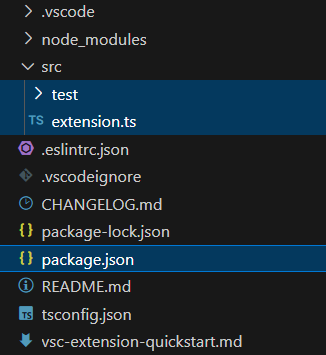
\includegraphics[width=.35\textwidth]{vscode_generated_structure}
    \caption{Durch \emph{Yeoman} generierte Ordnerstruktur.}
    \label{fig:vscode_generated_structure}
\end{figure}   

\subsection{Entwicklung}

\subsubsection{RecentChangeStorage}

Beim \emph{RecentChangeStorage}, 
der in Abbildung \ref{fig:diagram_VSCodeDesign-Detail_Storage} abgebildet ist,
handelt es sich um eine Klasse, die
von fast allen anderen Komponenten benötigt wird. Sie speichert ihre
Daten in einer sogenannten \emph{EvictingQueue}. Hierfür gibt es in
TypeScript keine mitgelieferte Implementierung, allerdings kann
diese sehr einfach über die Methode \emph{.shift()} eines Arrays
nachgebaut werden. So werden Elemente am Ende der Schlange automatisch
wieder entfernt, sobald sich die Schlange füllt. 
In der gespeicherten Warteschlange werden
Objekte der Klasse \emph{SimpleDiff} gespeichert. Diese bilden jeweils
eine Änderung ab, indem sie den entfernten und den ersetzenden Text
speichern. Der Zugriff auf die \emph{EvictingQueue}, also das Hinzufügen, 
das Auslesen und das Verändern der Anzahl von gespeicherten
Änderungen, wird durch verschiedene Methoden bereitgestellt.
Zusätzlich ist relevant, dass \emph{RecentChangeStorage} von der
Schnittstelle \emph{EventTarget} ableitet. Durch solche Events
kann ein Observer Pattern implementiert werden. Das \emph{storageChanged}
Event wird dabei immer ausgelöst, wenn sich der Inhalt der Warteschlange
verändert. Initialisiert wird der \emph{RecentChangeStorage} zu Beginn der
Methode \emph{activate}, in der Datei \emph{extension.ts}. So kann
das erstellte Objekt allen anderen Komponenten über den Konstruktor
übergeben werden.

\begin{figure}
    \centering
    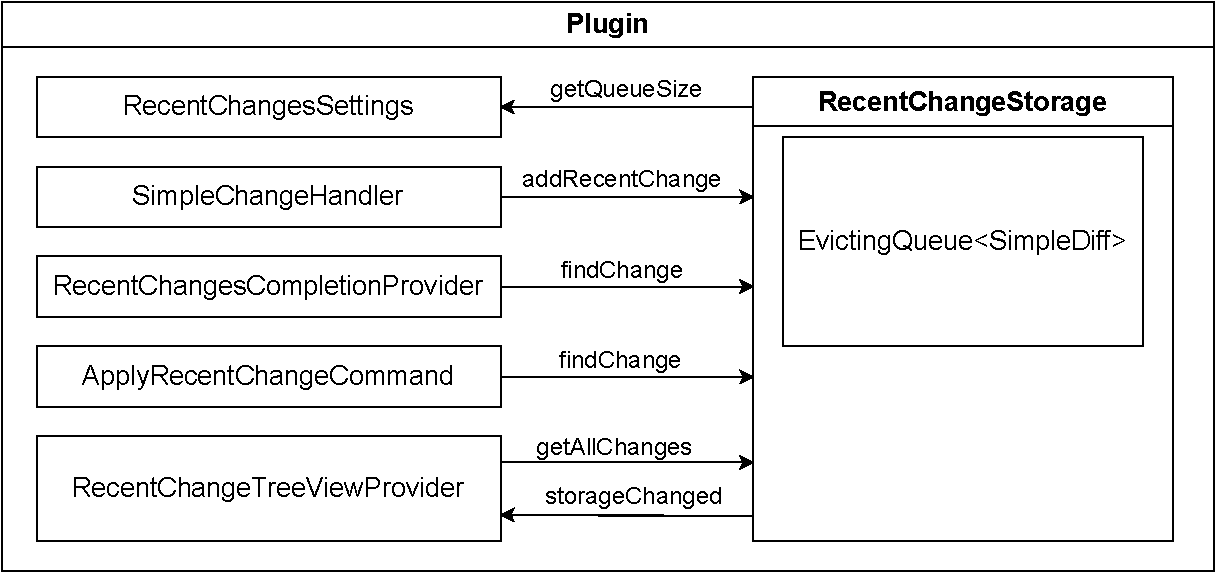
\includegraphics[width=.70\textwidth]{diagram_VSCodeDesign-Detail_Storage}
    \caption{Detaillierte Darstellung des \emph{RecentChangeStorage}.}
    \label{fig:diagram_VSCodeDesign-Detail_Storage}
\end{figure}   

\subsubsection{SimpleChangeHandler}

Der \emph{SimpleChangeHandler}, 
dessen Aufbau auch in Abbildung \ref{fig:diagram_VSCodeDesign-Detail_Handler} ersichtlich ist,
enthält mehrere Listener-Methoden,
die das Öffnen von Dateien, das Bearbeiten von Dateien und das
Wechseln des aktiven Editors beobachten. Diese Listener werden
in der Methode \emph{activate} registriert. Durch diese Listener
kann der aktuelle Zustand der geöffneten Datei, sowie ihr Zustand
zu Beginn einer Änderung, ständig beobachtet werden. Während
die NutzerInnen die Datei bearbeiten, wird immer wieder ein
Timer gestartet. Erst wenn der Timer, ohne einer Eingabe
in der Zwischenzeit, abläuft wird eine Änderung registriert. Auf diese 
Weise wird ein Debounce-Effekt erzeugt. Sobald eine Änderung
registriert wurde, werden der Ausgangszustand und der neue Zustand
der Datei verglichen. Hierfür wird Googles 
\emph{diff-match-patch}-Algorithmus \cite{DiffMatchPatchGithub}
verwendet, der auch komplexe Veränderungen in Texten erkennen kann. 
Immer wenn durch den Algorithmus eine einfache Veränderung gefunden
wurde, wird diese in Form eines \emph{SimpleDiff}-Objekts in
den \emph{RecentChangeStorage} eingefügt.

\begin{figure}
    \centering
    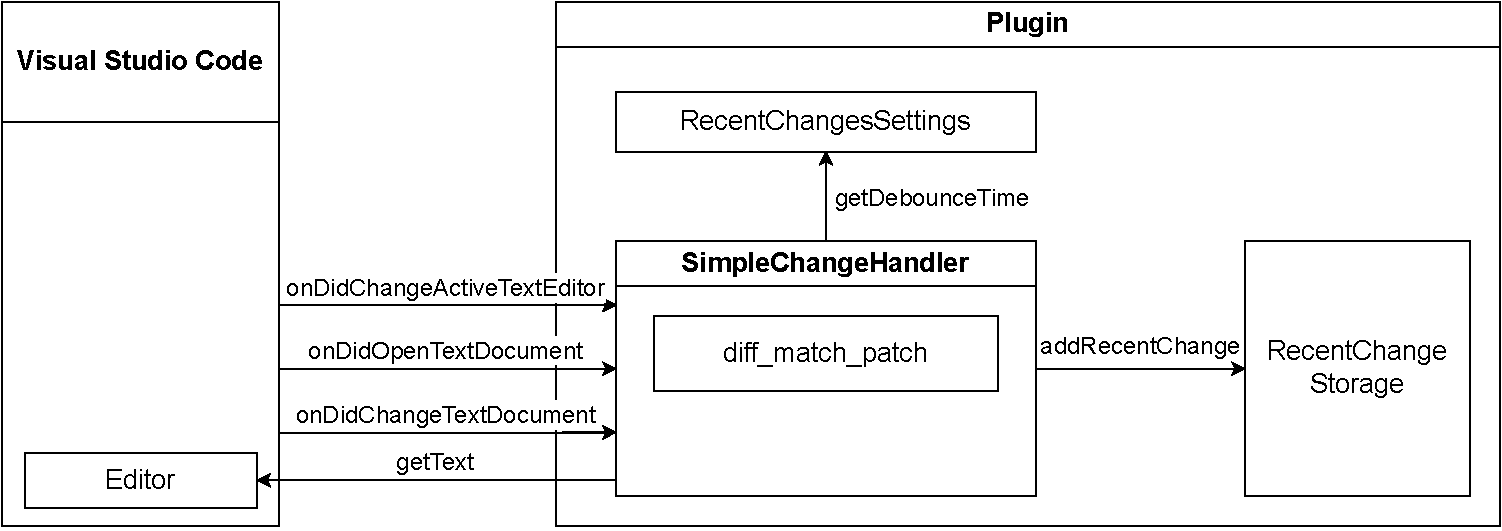
\includegraphics[width=.95\textwidth]{diagram_VSCodeDesign-Detail_Handler}
    \caption{Detaillierte Darstellung des \emph{SimpleChangeHandler}.}
    \label{fig:diagram_VSCodeDesign-Detail_Handler}
\end{figure}

\subsubsection{ApplyRecentChangeCommand}

Der \emph{ApplyRecentChangeCommand}, 
der in Abbildung \ref{fig:diagram_VSCodeDesign-Detail_Command} gefunden werden kann,
enthält eine einfache Methode,
die bei Aktivierung des Commands aufgerufen wird. Sie prüft zuerst
einfache Bedingungen, zum Beispiel, ob ein Editor aktiv ist.
Danach selektiert sie Mithilfe der Methode \emph{getWordRangeAtPosition},
welche von der VS Code API bereitgestellt wird, das zu ersetzende Wort.
Für dieses Wort wird der \emph{RecentChangeStorage} nach einer passenden
Änderung durchsucht. Wird diese gefunden, so werden die zu ersetzenden
Positionen berechnet und dann im Editor ersetzt. Um den Command auch 
verwendbar zu machen, müssen zusätzlich ein Command und ein Keybinding
in der Datei \emph{package.json} registriert werden. Die Zuordnung
der auszuführenden Methode erfolgt in der Methode \emph{activate}
durch Registrierung.

\begin{figure}
    \centering
    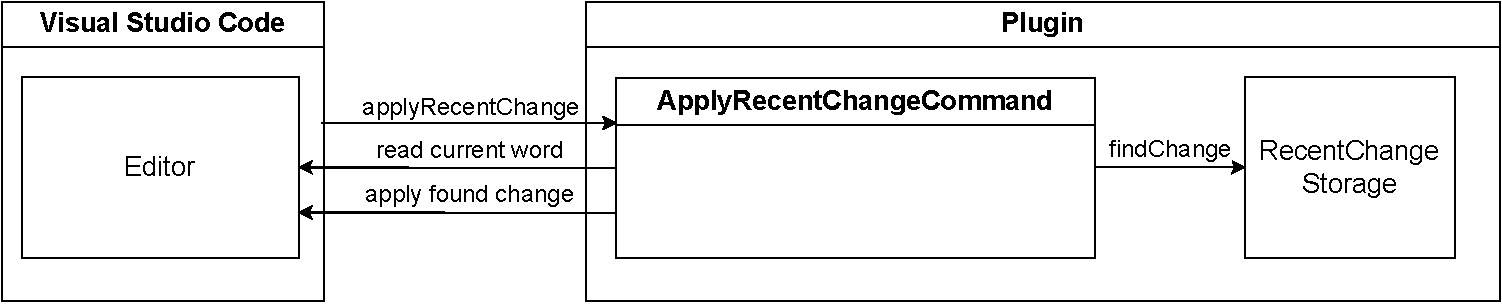
\includegraphics[width=.95\textwidth]{diagram_VSCodeDesign-Detail_Command}
    \caption{Detaillierte Darstellung des \emph{ApplyRecentChangeCommand}.}
    \label{fig:diagram_VSCodeDesign-Detail_Command}
\end{figure}   

\subsubsection{RecentChangesCompletionProvider}

Die Logik des \emph{RecentChangesCompletionProvider}, 
der in Abbildung \ref{fig:diagram_VSCodeDesign-Detail_Provider} dargestellt wird,
ist ähnlich
zu der des \emph{ApplyRecentChangeCommand}, da im Grunde nur für
die aktuelle Position im Editor nach einer passenden Änderung 
gesucht wird. Allerdings muss die Änderung hier nicht sofort
angewendet werden, sondern nur, in Form von \emph{CompletionItem}-Objekten,
retourniert werden. Das Registrieren des Providers wird durch
Aufruf der Methode \emph{activateRecentChangesCompletionProvider} bei
der Aktivierung des Plugins erledigt. Hier muss bei der Registrierung
auch ein Pattern für die Dateien angegeben werden, auf die der Provider
anwendbar ist.

\begin{figure}
    \centering
    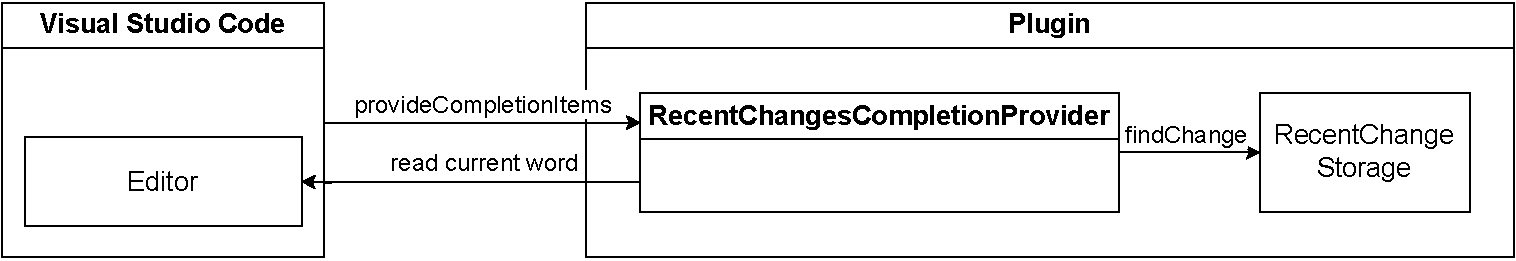
\includegraphics[width=.95\textwidth]{diagram_VSCodeDesign-Detail_Provider}
    \caption{Detaillierte Darstellung des \emph{RecentChangesCompletionProvider}.}
    \label{fig:diagram_VSCodeDesign-Detail_Provider}
\end{figure}   

\subsubsection{RecentChangeTreeViewProvider}

Das TreeView wird vom \emph{RecentChangeTreeViewProvider} bereitgestellt,
der in Abbildung \ref{fig:diagram_VSCodeDesign-Detail_TreeView} abgebildet ist.
Um das TreeView bereitzustellen, muss die Schnittstelle
\emph{TreeDataProvider<T>} implementiert werden. Diese
enthält eine Methode um alle Kinder eines \emph{T}-Elements
zu erhalten und eine Methode um ein \emph{T}-Element in
ein \emph{TreeItem} umzuwandeln. Um die zweite Methode etwas zu
vereinfachen, kann eine Klasse \emph{SimpleDiffTreeItem} direkt
von \emph{TreeItem} abgeleitet werden. Jedes TreeItem definiert
bestimmte Werte wie zum Beispiel eine Beschriftung (\emph{label}), 
ein Symbol (\emph{iconPath}) oder einen Hinweis (\emph{tooltip}).
Die \emph{SimpleDiffTreeItem}-Objekte enthalten zusätzliche
Metainformationen über ihre Position im Baum. Um die Baumstruktur
neu zu laden, kann das Event \emph{\_onDidChangeTreeData} aktiviert
werden. Dies muss immer dann passieren, wenn vom \emph{RecentChangeStorage}
das \emph{storageChanged} Event gefeuert wird.
Um die TreeView auch anzuzeigen, müssen in der Datei \emph{package.json}
sowohl ein ViewContainer als auch eine dazugehörige View registriert werden.
In der Methode \emph{activate} wird die Provider-Klasse mittels
des Aufrufes von \emph{vscode.window.createTreeView} dem registrierten
View zugeordnet.

\begin{figure}
    \centering
    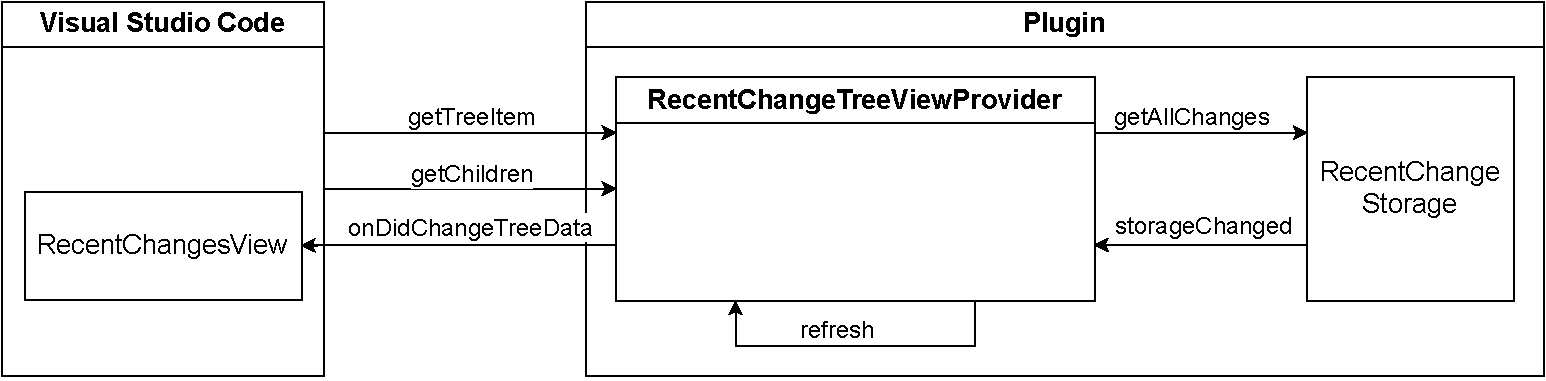
\includegraphics[width=.95\textwidth]{diagram_VSCodeDesign-Detail_TreeView}
    \caption{Detaillierte Darstellung des \emph{RecentChangeTreeViewProvider}.}
    \label{fig:diagram_VSCodeDesign-Detail_TreeView}
\end{figure}   

\subsubsection{RecentChangesSettings}

Die Einstellungen der Extension werden hauptsächlich in der Datei
\emph{package.json} festgelegt. Hier werden die Namen, Typen, 
Beschreibungen und Standardwerte der einzelnen Einstellungen bestimmt.
Die Klasse \emph{RecentChangesSettings} enthält nur statische 
Methoden, welche das Auslesen der Einstellungen übernehmen und
von überall im Code aufgerufen werden können.
Diese Klasse ist auch in der Abbildung \ref{fig:diagram_VSCodeDesign-Detail_Settings} 
ersichtlich.

\begin{figure}
    \centering
    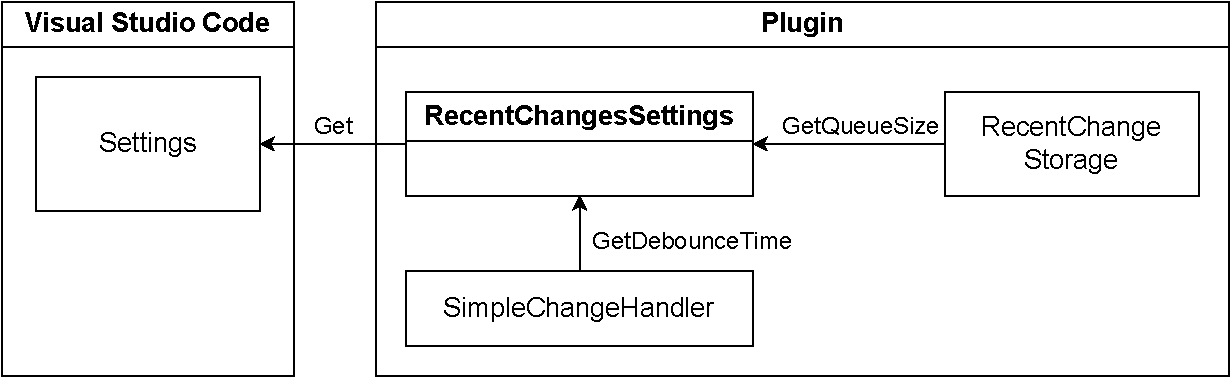
\includegraphics[width=.95\textwidth]{diagram_VSCodeDesign-Detail_Settings}
    \caption{Detaillierte Darstellung der Komponente \emph{RecentChangesSettings}.}
    \label{fig:diagram_VSCodeDesign-Detail_Settings}
\end{figure} 

\section{Tests}
\label{sec:EntwicklungVsCode_Tests}

Beim Erstellen einer neuen Extension wird im Ordner \emph{src} 
auch automatisch ein Ordner \emph{test} angelegt. 
In den generierten Dateien befindet sich 
eine Konfiguration für das Test\-framework Mocha \cite{MochaJSWebsite}, 
die bereits zur Ausführung bereite Tests enthält. Natürlich
kann Mocha auch mit jedem anderen, programmatisch ausführbaren,
TestFramework ersetzt werden. Die Testfälle nutzen eine Schnittstelle
aus dem Paket \emph{@vscode/test-electron} \cite{VSCodeTestElectronGithub}. 
Diese führt die Tests
innerhalb einer speziellen Instanz von VS Code namens 
\emph{Extension Development Host} aus. Auf diese Weise kann auch
während der Tests auf das Modul \emph{vscode} zugegriffen werden.
Dadurch ist es nicht nur möglich einfache Unit-Tests zu entwickeln, 
sondern es können auch größer angelegte Integrationstests
geprüft werden, die eine Interaktion mit VS Code benötigen 
\cite{VSCodeExtensionAPITestingExtensions}.

\section{Publishing}
\label{sec:EntwicklungVsCode_Publishing}

Das Veröffentlichen einer VS Code Extension funktioniert über das 
\emph{vsce} Komandozeilenwerkzeug. Dieses kann mithilfe des Befehls
\begin{GenericCode}[numbers=none]
npm install -g @vscode/vsce
\end{GenericCode}
installiert werden. Das fertige Plugin kann daraufhin mit 
\begin{GenericCode}[numbers=none]
vsce package
\end{GenericCode}
verpackt und mit 
\begin{GenericCode}[numbers=none]
vsce publish
\end{GenericCode}
in den VS Code Marketplace hochgeladen werden \cite{VSCodeExtensionAPIPublishingExtension}.

Beim Hochladen ist zu beachten, dass ein \emph{personal access token}
und ein \emph{publisher} Name benötigt werden.
Um den Token zu erhalten, muss man zuerst in Azure DevOps eine neue Organisation
anlegen (sofern man nicht bereits Teil einer Organisation ist). In den 
Benutzereinstellungen kann ein neuer Token erstellt werden. Dabei müssen auch die 
Berechtigungen für den Token festgelegt werden. Bei dem Abschnitt für 
\emph{Marketplace} muss hier die Berechtigung \emph{Manage} gesetzt sein.
Ein Publisher kann erstellt werden, indem man sich im Marketplace anmeldet
und die Seite \url{https://marketplace.visualstudio.com/manage} aufruft.
Hier gibt es einen Dialog zum Erstellen eines neuen Publishers. Dieser
Publisher benötigt mindestens eine eindeutige ID und einen eindeutigen
Namen, welche später im Marketplace angezeigt werden. Der Publisher Name
muss weiters noch in der Datei \emph{package.json} eingetragen werden.

Das Verwalten von bereits hochgeladenen Extensions kann entweder
über das Werkzeug \emph{vsce} oder über die grafische Benutzeroberfläche
im Marketplace erledigt werden.

\section{CI/CD}
\label{sec:EntwicklungVsCode_CICD}

Die Einbindung von automatisiertem Testen und Veröffentlichen
einer VS Code Extension ist sehr unkompliziert, da es hierzu
ausführliche Dokumentation gibt. Die Dokumentation bietet
weiters vorgefertigte Beispiele für Azure Pipelines, 
GitHub Actions, GitLab CI und Travis CI \cite{VSCodeExtensionAPIContinuousIntegration}.

Im Zuge der Entwicklung wurde mit GitHub Actions gearbeitet.
Der vorgeschlagene Workflow testet die Anwendung dabei unter
MacOS, Ubuntu und Windows. Beim automatischen Deployment muss
beachtet werden, dass in der Datei \emph{package.json} im
Abschnitt \emph{"scripts"} die zusätzliche Zeile
\begin{JsCode}[numbers=none]
"deploy": "vsce publish"
\end{JsCode}
nötig ist. Weiters muss beachtet werden, dass auch der zuvor erstellte 
\emph{personal access token} benötigt wird
(wie beschrieben in Abschnitt \ref{sec:EntwicklungVsCode_Publishing}).
Dieser muss im Workflow als Umgebungsvariable gesetzt werden und
wird, im Falle von GitHub Actions, am Besten als verschlüsseltes
\emph{secret} gespeichert.